\documentclass[10pt,a4paper]{article}
\usepackage{amsmath}
\usepackage{amssymb}
\usepackage{graphicx}
\usepackage{color}
\usepackage{fancyhdr}
\usepackage{fancyvrb}
\usepackage[margin=3.5cm]{geometry}
\usepackage{framed}
\usepackage{enumerate}
\usepackage{textcomp}
\def\ket#1{\left|#1\right\rangle}
\def\bra#1{\left\langle#1\right|}
\def\braket#1{\left\langle#1\right\rangle}
\usepackage{framed}

\definecolor{linkcol}{rgb}{0.0, 0.0, 0.5}
\usepackage[colorlinks=true,urlcolor=linkcol,citecolor=black,linkcolor=linkcol]{hyperref}

\renewcommand\thesection{1.\arabic{section}}
\renewcommand\thesubsection{\thesection.\arabic{subsection}}

\fancyhf{}
\lhead{\tiny Y.~D.~Chong (2016)}
\rhead{\scriptsize MH2801: Complex Methods for the Sciences}
\lfoot{}
\rfoot{\thepage}
\pagestyle{fancy}

\makeatletter
\def\PY@reset{\let\PY@it=\relax \let\PY@bf=\relax%
    \let\PY@ul=\relax \let\PY@tc=\relax%
    \let\PY@bc=\relax \let\PY@ff=\relax}
\def\PY@tok#1{\csname PY@tok@#1\endcsname}
\def\PY@toks#1+{\ifx\relax#1\empty\else%
    \PY@tok{#1}\expandafter\PY@toks\fi}
\def\PY@do#1{\PY@bc{\PY@tc{\PY@ul
\def\PYZdl{\char`\$}
\def\PYZhy{\char`\-}
\def\PYZsq{\char`\'}
\def\PYZdq{\char`\"}
\def\PYZti{\char`\~}

\begin{document}
\setcounter{page}{7}
\noindent
\underline{\textbf{\LARGE 1. Derivatives}}
\vskip 0.1in

The \textbf{derivative} of a function $f(x)$ is another function,
defined in terms of a limiting expression:

\begin{equation}
f'(x) \equiv \frac{df}{dx}(x) \equiv \lim_{\delta x \rightarrow 0} \, \frac{f(x + \delta x) - f(x)}{\delta x}.
\label{define_deriv}
\end{equation}
If the limiting expression give a unique and well-defined result
within some domain of $x$, then we say that the derivative ``exists''
in that domain. We also say that $f(x)$ is \textbf{differentiable} in
that domain. It can be shown that a differentiable function is
automatically continuous.  (Try proving it!) For the purposes of
dimensional analysis, the derivative of a function $f(x)$ has the
units of the original function, divided by the units of $x$.

\begin{figure}[h]
  \centering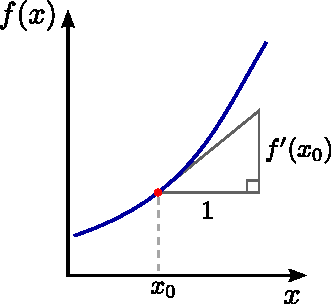
\includegraphics[width=0.32\textwidth]{derivative}
\end{figure}
    
Second-order and higher-order derivatives are defined by repeating the
derivative procedure. Graphically, the derivative represents the
``slope'' of the graph of $f(x)$, while the second derivative
represents the ``curvature''. For example, the graph above has
positive second derivative, because it is upward-curving.

 Derivatives obey several elementary composition rules:
\begin{align}
\frac{d}{dx}\left[\alpha\, f(x) + \beta\, g(x)\right] &= \alpha\, f'(x) + \beta\, g'(x) \quad &\textrm{(linearity)}& \\   \frac{d}{dx}\left[f(x) \, g(x)\right] &= f(x) \, g'(x) + f'(x) \, g(x) &\textrm{(product}\;\textrm{rule)}& \\   \frac{d}{dx}\left[f(g(x))\right] &= f'(g(x)) \, g'(x) &\textrm{(chain}\;\textrm{rule)}&
\end{align}
These can all be proven by directly substituting into
Eq.~(\ref{define_deriv}), and taking appropriate orders of
limits. With the aid of these rules, we can prove various standard
results, such as the ``power rule'' for derivatives:
\begin{equation*}
  \frac{d}{dx} \big[x^a\big] = a x^{a-1}.
\end{equation*}

The linearity of the derivative operation has the important
implication that derivatives ``commute'' with sums, i.e.~you can move
them to the left or right of summation signs. For example, we can use
this to show that the exponential function is its own derivative:
\begin{equation}
  \frac{d}{dx} \left[\exp(x)\right] \,=\,
  \frac{d}{dx} \sum_{n=0}^\infty\frac{x^n}{n!}
  \,=\, \sum_{n=0}^\infty\frac{d}{dx} \, \frac{x^n}{n!} \,=\,
  \sum_{n=1}^\infty \frac{x^{n-1}}{(n-1)!} =\exp(x).
\end{equation}

Derivatives also ``commute'' with limit expressions. For example, we
can use this on the alternative definition of the exponential
function:
\begin{align}
  \begin{aligned}
  \frac{d}{dx} \left[\exp(x)\right] &= \frac{d}{dx} \lim_{n\rightarrow\infty} \left(1+\frac{x}{n}\right)^n = \lim_{n\rightarrow\infty} \frac{d}{dx} \left(1+\frac{x}{n}\right)^n \\ &= \lim_{n\rightarrow\infty} \left(1+\frac{x}{n}\right)^{n-1} \;= \exp(x)
  \end{aligned}
\end{align}

\section{Taylor series}
\label{taylor-series}

A function is \textbf{infinitely differentiable} if all orders of
derivatives are well-defined (i.e., first derivative, second derivative,
etc.). Not all functions behave this way: for example, $f(x) = |x|$
has a first derivative which is discontinuous at $x = 0$, which means
that it has no well-defined second derivative at that point.

If a function is infinitely differentiable, then near any point $x_0$
it can be written out in a \textbf{Taylor series}:
\begin{align}
  f(x) \;&=\; \sum_{n=0}^\infty \frac{(x-x_0)^n}{n!} \left[\frac{d^n}{dx^n} f\right](x_0) \\&=\; f(x_0) + (x-x_0)\, f'(x_0) + \frac{(x-x_0)^2}{2} f''(x_0) + \cdots
\end{align}
Here, the ``zeroth derivative'' refers to the function itself. The
Taylor series can be derived by assuming that $f(x)$ can be written
out as a general polynomial involving terms of the form $(x-x_0)^n$;
from the definition of the derivative, we can then obtain the
polynomial coefficients. Because we are only `'assuming'' the validity
of the the polynomial series, there is no guarantee that the Taylor
series converges to the true value for any value of $x$. For many
functions, the Taylor series converges only if $|x-x_0|$ is smaller
than a certain amount.

\subsection{Useful Taylor Series}
\label{series}

\begin{align}
  \frac{1}{1-x} &= 1 + x + x^2 + x^3 + \cdots\mathrm{for} \; |x| < 1 \\
  \ln(1-x) &= -x - \frac{x^2}{2} - \frac{x^3}{3} - \frac{x^4}{4} - \cdots \quad \mathrm{for} \; |x| < 1 \\
  \sin(x) &= x - \frac{x^3}{3!} + \frac{x^5}{5!} - \frac{x^7}{7!} + \cdots \\
  \sinh(x) &= x + \frac{x^3}{3!} + \frac{x^5}{5!} + \frac{x^7}{7!} + \cdots \\
  \cos(x) &= 1 - \frac{x^2}{2!} + \frac{x^4}{4!} - \frac{x^6}{6!} + \cdots \\
  \cosh(x) &= 1 + \frac{x^2}{2!} + \frac{x^4}{4!} + \frac{x^6}{6!} + \cdots
\end{align}

Apart from the first two, the others are actually exact for all $x$.
The sine and cosine functions and the hyperbolic functions are
``entire'', which means that their Taylor series converge everywhere
in the domain $\mathbb{R}$.  If you pick a large value of $x$,
however, you may have to sum to a very high order before the series
converges to an accurate value.

\section{Ordinary differential equations}
\label{ordinary-differential-equations}

A differential equation is an equation involving several different
derivatives of a function. For example,
\begin{equation}
\frac{df}{dx} = \kappa f(x)
\label{ode_ex}
\end{equation}
involves both $f(x)$ and its first derivative. Specifically, this is
an \textbf{ordinary differential equation}, because $f(x)$ is a
function involving a single input number $x$.

There is no single fixed procedure for solving differential equations.
In some cases, we can guess the solution: for example, we might happen
to know that the above differential equation has solutions of the form
\begin{equation}
  f(x) = A \exp(\kappa x).
  \label{ode_sol}
\end{equation}
There are methods, such as Green's functions, for generating solutions
to certain special classes of differential equation. But many
differential equations simply cannot be solved analytically, and can
only be solved numerically.

When confronted with an ordinary differential equation, typically the
first thing you should look for is the order of the highest derivative
appearing in the equation.  This is also called the \textbf{order} of
the differential equation. If the equation has order $N$, then its
\textbf{general solution} contains $N$ independent parameters, or
``constants of integration''.

Now, if you happen to be able to guess a solution to the equation, but
that solution does not contain $N$ parameters, then you know that your
solution isn't the most general one.  For example, in
Eq.~(\ref{ode_ex}), the order is 1.  We guessed the solution
(\ref{ode_sol}), which has one parameter $A$. So we know our work is
done: there is no solution more general than the one we found.

A \textbf{specific solution} to a differential equation is a solution in
which there are no independent parameters. This can be done by assigning
numerical values to the independent parameters of the general solution.
These numerical values are often specified in terms of ``boundary
conditions''. For example, for a second-order differential equation, I
might give you $f(x = 0)$ and $f'(x = 0)$, and ask you to find the
corresponding specific solution. Alternatively, I could give you
$f(x = 0)$ and $f(x = 1)$, or any other combination of two
conditions. For an ordinary differential equation of order $N$, we
need $N$ boundary conditions to arrive at a specific solution.

\begin{framed}
\noindent
\underline{\textbf{Example}}
\vskip 0.1in \noindent
The following differential equation describes a damped harmonic
oscillator:
\begin{equation}
  \frac{d^2 x}{dt^2} + 2\gamma\frac{dx}{dt} + \omega_0^2 x(t) = 0.
  \label{oscillator}
\end{equation}
In this case, note that $x(t)$ is the function, and $t$ is the input
variable.  This is unlike our previous notation where $x$ was the
input variable; don't get confused!

Eq.~(\ref{oscillator}) is obtained from Newton's second law, for an
object moving in one dimension subject to a damping force and a
restoring force. Thus $x(t)$ represents the position as a function of
time. We will come back to this equation when studying the damped
harmonic oscillator in greater detail.
\end{framed}

\section{Partial derivatives}
\label{partial-derivatives}

So far, we have focused on functions which take a single input.
Functions can also take multiple inputs; for instance, a function
$f(x,y)$ maps two input numbers, $x$ and $y$, and outputs a
number. In general, the inputs are allowed to vary independently of one
another. The \textbf{partial derivative} of such a function is its
derivative with respect to one of its inputs, keeping the other input
fixed. For example,
\begin{equation}
  f(x,y) = \sin(2x - 3 y^2)
\end{equation}
has partial derivatives
\begin{equation}
\frac{\partial f}{\partial x} = 2\cos(2x-3y^2), \quad \frac{\partial f}{\partial y} = - 6\cos(2x-3y^2).
\end{equation}

\subsection{Change of variables}
\label{change-of-variables}

We've seen that single-variable functions obey a derivative
composition rule
\begin{equation}
  \frac{d}{dx}\, f\big(g(x)\big) = g'(x) \, f'\big(g(x)\big).
\end{equation}
This composition rule has a important generalization for partial
derivatives, which is related to the physical concept of a
\textbf{change of coordinates}. Suppose we have a function $f(x,y)$
which takes two inputs $x$ and $y$, and wish to express them using a
different coordinate system denoted (say) $u$ and $v$. In general,
each coordinate in the old system would depend on `'both'' coordinates
in the new system:
\begin{equation}
  x = x(u,v), \quad y = y(u,v).
\end{equation}
Expressed in the new coordinates, the function is
\begin{equation}
F(u,v) \equiv f\big(x(u,v), y(u,v)\big).
\end{equation}
It can then be shown that this transformed function's partial
derivatives obey the composition rule
\begin{align}
  \frac{\partial F}{\partial u} &= \frac{\partial f}{\partial x} \frac{\partial x}{\partial u} + \frac{\partial f}{\partial y} \frac{\partial y}{\partial u}\\
  \frac{\partial F}{\partial v} &= \frac{\partial f}{\partial x} \frac{\partial x}{\partial v} + \frac{\partial f}{\partial y} \frac{\partial y}{\partial v}.
\end{align}
On the right-hand side of these equations, the partial derivatives are
to be expressed in terms of the new coordiantes $(u,v)$. For example,
\begin{equation}
  \frac{\partial f}{\partial x} = \left.\frac{\partial f}{\partial x}\right|_{x = x(u,v), \;y= y(u,v)}
\end{equation}
The generalization of this rule to more than two inputs is
straightforward. For a function $f(x_1, \dots, x_N)$, a change of
coordinates $x_i = x_i(u_1, \dots, u_N)$ involves the composition
\begin{equation}
F(u_1, \dots, u_N) = f\big(x_1(u_1,\dots,u_N\big), \dots), \quad \frac{\partial F}{\partial u_i} = \sum_{j=1}^N \frac{\partial x_j}{\partial u_i} \frac{\partial f}{\partial x_j}.
\end{equation}

\begin{framed}
\noindent
\underline{\textbf{Example}}
\vskip 0.1in \noindent
In two dimensions, Cartesian and polar coordinates are related by the
formulas
\begin{equation}
x = r\cos\theta, \quad y = r\sin\theta.
\end{equation}
If we have a function $f(x,y)$, we can re-write it in polar
coordinates as $F(r,\theta)$.  The partial derivatives are related by
\begin{align}
  \frac{\partial F}{\partial r} &=
  \frac{\partial f}{\partial x} \frac{\partial x}{\partial r} + \frac{\partial f}{\partial y} \frac{\partial y}{\partial r} = \frac{\partial f}{\partial x} \cos\theta + \frac{\partial f}{\partial y} \sin\theta. \\
  \frac{\partial F}{\partial \theta} &= \frac{\partial f}{\partial x} \frac{\partial x}{\partial \theta} + \frac{\partial f}{\partial y} \frac{\partial y}{\partial \theta} = -\frac{\partial f}{\partial x} r\,\sin\theta + \frac{\partial f}{\partial y} r\cos\theta.
\end{align}
This is often written in matrix form as:
\begin{equation}
  \begin{bmatrix}\partial F/\partial r \\ (1/r) \,
  \partial F/\partial \theta\end{bmatrix}
  = \begin{bmatrix}\cos(\theta) & \sin(\theta)\\ -\sin(\theta) &
    \cos(\theta) \end{bmatrix}\, \begin{bmatrix}\partial f/\partial x
    \\ \partial f/\partial y\end{bmatrix}.
\end{equation}
\end{framed}

\subsection{Partial differential equations}
\label{partial-differential-equations}

A partial differential equation is a differential equation which
involves multiple partial derivatives (as opposed to an
\emph{ordinary} differential equation, which involves only derivatives
with respect to a single variable). An example of a partial
differential equation is Laplace's equation,
\begin{equation}
\frac{\partial^2 \Phi}{\partial x^2} + \frac{\partial^2 \Phi}{\partial y^2} + \frac{\partial^2 \Phi}{\partial z^2}= 0,
\end{equation}
which describes the electrostatic potential $\Phi(x,y,z)$ at position
$(x,y,z)$, in the absence of any electric charges. Partial
differential equations are significantly harder to solve than ordinary
differential equations. For example, boundary conditions are more
complicated to specify: whereas each boundary condition for an ordinary
differential equation consists of a single number (e.g., the value of
$f(x)$ at some point $x = x_0$), each boundary condition for a
partial differential equation consists of a \emph{function} (e.g., the
values of $\Phi(x,y,z)$ along some curve $g(x,y,z) = 0$).

\section{Exercises}\label{exercises}

\begin{enumerate}
\item 
  Prove that
  \begin{equation}
\frac{d}{dx} [x^y] = y x^{y-1}, \quad\mathrm{for}\;\;x \in \mathbb{R}^+, \; y \notin \mathbb{N},
  \end{equation}
  starting from the previously-discussed definition of non-natural
  powers, in terms of the exponential and logarithm functions.

\item
  Consider $f(x) = \tanh(\alpha x)$.  Sketch $f(x)$ versus $x$, for
  two cases: (i) $\alpha = 1$ and (ii) $\alpha \gg 1$.  Sketch the
  derivative function $f'(x)$ for the two cases, based on your
  sketches in part (a) (i.e., without evaluating the derivative
  directly).  Evaluate the derivative function, and verify that the
  result matches your sketches in part (b).

\item
  Prove geometrically that the derivatives of the sine and cosine
  functions are:
  \begin{equation} \frac{d}{dx}\sin(x) = \cos(x),
    \quad\frac{d}{dx}\cos(x) = -\sin(x).
  \end{equation}
  Hence, derive their \hyperref[series]{series expansions}.

\item
  For each of the following functions, derive the Taylor series around
  $x = 0$:
  \begin{itemize}
  \item 
    $f(x) = \ln\left[\alpha \cos(x)\right]$, to the first 3 non-vanishing terms.
  \item
    $f(x) = \cos\left[\pi\exp(x)\right]$, to the first 4 non-vanishing terms.
  \item
    $\displaystyle f(x) = \frac{1}{\sqrt{1 \pm x}}$, to the first 4 non-vanishing terms.  Keep track of the signs (i.e., $\pm$ versus $\mp$).
  \end{itemize}
  
\item
For each of the following functions, sketch the graph and state the
domains over which the function is differentiable:
\begin{itemize}
\item $\displaystyle f(x) = |\sin(x)|$
\item $\displaystyle f(x) = \left[\tan(x)\right]^2$
\item $\displaystyle f(x) = \frac{1}{1-x^2}$
\end{itemize}

\item
  Let $\vec{v}(x)$ be a ``vectorial'' function which takes an input
  $x$ (a number), and gives an output value $\vec{v}$ that is a
  2-component vector. The derivative of this vectorial function is
  defined in terms of the derivatives of each vector component:
\begin{equation}
\vec{v}(x) = \begin{bmatrix}v_1(x) \\ v_2(x)\end{bmatrix} \;\; \Rightarrow \;\; \frac{d\vec{v}}{dx} = \begin{bmatrix}dv_1/dx \\ dv_2/dx\end{bmatrix}.
\end{equation}
Now suppose $\vec{v}(x)$ obeys the vectorial differential equation
\begin{equation}
\frac{d\vec{v}}{dx} = \mathbf{A} \vec{v}, \quad\mathrm{where}\;\;\mathbf{A} = \begin{bmatrix}A_{11} & A_{12} \\ A_{21} & A_{22}\end{bmatrix}.
\end{equation}
How many independent numbers do we need to specify for the general
solution?

Next, let $\vec{u}$ be one of the eigenvectors of $\mathbf{A}$, with
eigenvalue $\lambda$:
\begin{equation}
\mathbf{A} \vec{u} = \lambda \vec{u}.
\end{equation}
Show that $\vec{v}(x) = \vec{u}\, e^{\lambda x}$ is a specific
solution to the vectorial differential equation. Hence, find the general
solution.

\item
  Show that if a function is differentiable, then it is also
  continuous.
\end{enumerate}
\end{document}
